
% ===========================================================================
% Title:
% ---------------------------------------------------------------------------
% to create Type I fonts type "dvips -P cmz -t letter <filename>"
% ===========================================================================
\documentclass[11pt]{article}       %--- LATEX 2e base
\usepackage{amsmath}
\usepackage[utf8]{inputenc}
\usepackage{latexsym}               %--- LATEX 2e base
\usepackage{algorithm2e}
\usepackage{hyperref}
\newcommand{\Mod}[1]{\ (\mathrm{mod}\ #1)}
\usepackage{subcaption}
\usepackage[none]{hyphenat}
%---------------- Wide format -----------------------------------------------
\textwidth=6in \textheight=9in \oddsidemargin=0.25in
\evensidemargin=0.25in \topmargin=-0.5in
%--------------- Def., Theorem, Proof, etc. ---------------------------------
\newtheorem{definition}{Definition}
\newtheorem{theorem}{Theorem}
\newtheorem{lemma}{Lemma}
\newtheorem{corollary}{Corollary}
\newtheorem{property}{Property}
\newtheorem{observation}{Observation}
\newtheorem{fact}{Fact}
\newenvironment{proof}           {\noindent{\bf Proof.} }%
                                 {\null\hfill$\Box$\par\medskip}


\usepackage{graphicx}

\newcommand{\includeFig}[3]      {\begin{figure}[htb] \begin{center}
                                 \includegraphics
                                 [width=4in,keepaspectratio] %comment this line to disable scaling
                                 {#2}\caption{\label{#1}#3} \end{center} \end{figure}}
                                 % usage: \includeFig{label}{file}{caption}

\SetKwComment{Comment}{/* }{ */}

\RestyleAlgo{ruled}

% ===========================================================================
\begin{document}
% ===========================================================================

% ############################################################################
% Title
% ############################################################################

\title{A Parallel Jacobi Gauss-Seidel Method with Dynamic Parallelization}


% ############################################################################
% Author(s) (no blank lines !)
\author{
% ############################################################################
Nirav C. Pansuriya\\
School of Computer Science\\
Carleton University\\
Ottawa, Canada K1S 5B6\\
{\em niravchhaganbhaipan@cmail.carleton.ca}
% ############################################################################
} % end-authors
% ############################################################################

\maketitle

% ############################################################################
% Abstract
% ############################################################################
\begin{abstract}
Methods for solving large system of linear equations have always been a topic of interest for researchers.  The Jacobi and Gauss-Seidel methods are both very well-known methods for solving linear equations. While the Jacobi method is easy to implemented in a parallel environment, it is extremely slow at solving equations; on the other hand, the GS method is extremely quick at solving equations but extremely complex to implement in a parallel environment. To address this issue, the PJG (Parallel Jacobian Gauss-Seidel Method) was introduced. This method is capable of solving large system of linear equations in small number of iterations and is extremely simple to apply in a parallel environment too. The primary objective of this research is to further enhance the performance of the PJG method by implementing the concept of dynamic parallelization. Additionally, performance of the proposed method (PJG method with dynamic parallelization) is compared with the Jacobi method, the GS method, and the PJG method by implementing these algorithms in a parallel system.
\end{abstract}

% ############################################################################
\section{Introduction} \label{introduction}
% ############################################################################

Computer architecture has become increasingly parallel in recent years. Modern GPUs, such as the NVIDIA GForce GTX 280 provide enormous parallelism. So, the focus of researchers has moved to parallelism rather than continuous improvements to the single unit speed of computation. We regularly encounter several linear systems in physics, mathematics, and engineering. In many scientific simulations, we have to solve large-scale linear equations. However, large-scale linear equations require a significant amount of time and resources, such as memory. It is always a trending topic among researchers to find an algorithm that can solve large-scale linear equations in less time and with fewer resources. Many scientific methods, such as iterative and direct methods, exist for solving large-scale, computationally expensive linear systems of equations. When solving large systems of linear equations, iterative methods are typically preferred over direct methods. This is because direct methods are very computationally expensive for large linear systems, while iterative methods require lower memory and shorter execution times. The Jacobi and Gauss-Seidel methods are two famous and well-known iterative methods for solving systems of linear equations. Although the Jacobi approach is extremely simple to implement in a parallel environment, it requires an excessive number of iterations to solve a large system of linear equations. The Gauss-Seidel method is an improved version of the Jacobi method. The GS method is capable of solving a large system of linear equations in a small number of iterations. However, because this method is sequential in nature, it is extremely difficult to implement in a parallel environment. One method is easily implemented in a parallel environment but requires an excessive number of iterations to solve, whereas the other method can solve a large system of linear equations in a very few iterations but cannot be implemented in a parallel environment. To address this issue, the PJG (Parallel Jacobian Gauss-Seidel Method) was introduced. This method is capable of solving large systems of linear equations in a small number of iterations and is extremely simple to apply in a parallel environment too. The primary objective of this research is to further enhance the performance of the PJG method by implementing the concept of dynamic parallelization. I compared the proposed method (PJG method with dynamic parallelization) with the Jacobi method, the GS method, and the PJG method. I implemented all of these algorithms in CUDA and executed them on a GPU in order to compare their performance with the proposed technique. Among the Jacobi method, the GS method, and the PJG method, the PJG method took the least time to solve a large system of linear equations. The PJG method achieved up to a 7x faster speed compared to the GS method. I solved the same system of linear equations using my proposed method. Results indicate an improvement in runtime, reaching up to a 10x faster speed compared with the GS method and up to a 1.3x faster speed compared with the PJG method.


% ############################################################################
\section{Literature Review} \label{litrev}
% ############################################################################

Large linear equation systems are used in many complex scientific simulators. Solving such huge systems requires a significant amount of processing resources, such as memory and CPU. Solving a large system of linear equations is a very time consuming procedure. That is why developing effective algorithms to solve such big systems in a limited amount of time and with limited resources is always a research interest.
\\
\\
There are two approaches to solving linear equations: a direct approach and an iterative approach. In a direct approach,  equations are solved in finite steps, but the time complexity is $O(n^{3})$ \cite{numerical-mathematics}, which is quite high when the system of linear equations is large. This is because direct approaches scale intensively with respect to the size of system of linear equations. The indirect technique has a time complexity of $O(n^2)$. The variables in the linear equation are initially initialized with random values in an indirect way. Following that, we find a close approximation with each iteration. Additionally, indirect approaches consume less memory and resources than direct approaches. That is why the majority of research is conducted using iterative approaches, as they need fewer computational resources than direct methods.
\\
\\
The Jacobi method and the Gauss-Seidel method are two well-known iterative approaches. \cite{hageman2016applied}. Both methods are used to solve linear equations represented in matrix form. Any system of linear equations can be  $AX = B$, where $A$ is the coefficent matrix, $B$ is a vector of competitors, and $X$ is a vector of variables. In the Jacobi method, variables (vector $X$) initialised with random values. In the Jacobi method, variables (vector $X$) initialised with random values. After that, to solve each diagonal element in matrix A, values of variables (vector $X$) are plugged into the linear equation.  By doing this, the new values of variables are calculated.  All of these steps are repeated until convergence occurs. The   Gauss-Seidel method is similar to the Jacobi method. The only difference is that variables in the Jacobi approach are updated after each iteration, but variables in the GS method are updated immediately after each diagonal element is solved. That is why, in comparison to the Jacobi method, the GS method has a higher convergence speed. The only disadvantage of the GS method is that it is very hard to implement in parallel systems compared to the Jacobi method, because the GS method is sequential in nature.
\\
\\
There are many parallel algorithms for the GS method. The Red-Black GS algorithm is very popular \cite{rbgs}. This algorithm is based on the ordering of multiple colours. The specific matrix structure require to work this this method, and so it is dependent on the sparsity pattern of a matrix. As a result, we cannot use it with all systems of linear equations.
\\
\\
In the paper \cite{row-based}, the author has come up with a row-based parallel method. This method is derived from the GS method. To solve every diagonal element, we do the multiplication of constants and current variables. For each linear equation, this method performs all of these multiplication operations simultaneously in a parallel environment. After all these multiplication operations are completed for a full row of matrix $A$, variables get updated. This procedure is repeated until convergence occurs.
\\
\\
In paper \cite{base-paper}, the author has come up with a new parallel method to solve linear equations by combining two other algorithms. This new method can achieve a good parallelization and can solve large systems of linear equations in very few iterations. The author has merged the Jacobi method's parallelism with the GS method's rapid convergence. The main advantage of this method is that there is no need to have any special pattern in matrix. And so this method can work with a sparse matrix as well as a dense matrix. In this new approach, linear equations are divided into blocks. Every equation within the same block is solved in a parallel environment at the same time, as the Jacobi method is very easy to implement in a parallel environment. After that, variables get updated as one would do in the GS method, and equations within the next block will use the updated values of variables. This new approach is called the PJG method. This method is being improved in this research work.

% ############################################################################
\section{Algorithms} \label{algos}
% ############################################################################

% ############################################################################
\subsection{Jacobi Method (Sequential version)}
% ############################################################################

The Jacobi method is a well-known iterative method for solving system of linear equations\cite{2013handbook}. The Jacobi method is based on the following principle: take an equation and arrange it in terms of $X_{n+1} = F(X_n)$. By initializing $X_n$ with some value and then plugging it into the $F(X_n)$ equation, a new value $X_{n+1}$ is calculated and then it is used as the next $X_n$ value. These operations are repeated until convergence is achieved. During this iterative process, when the value of variable $X_n$ is set such a way that both sides of the linear equation are nearly equal, one can say that convergence has achieved.

\begin{algorithm}
\DontPrintSemicolon
\caption{Convergence}\label{alg:convergence}
\SetKwInOut{Input}{input}
\SetKwInOut{Output}{output}
\Input{matrix A = coefficient matrix\\ vector X = variables\\ vector B = constant vector  }
\Output{whether convergence is achived or not}
$error \gets 0$\;
\For{$i \gets 0$ \KwTo $size$}{
    $prediction \gets 0$\;
    \For{$j \gets 0$ \KwTo $size$}{
         $prediction \gets predction + A[i][j] \times X[j]$\;
    }
    $error \gets error + |prediction - B[i]|$  \Comment*[r]{absolute value}
}
\eIf{$error \leq threshold$}{
     \texttt{convergence is true}
}{
    \texttt{convergence is false}
}
\end{algorithm}


\begin{algorithm}
\DontPrintSemicolon 
\caption{Jacobi (Sequential)}\label{alg:jacobi_seq}
\SetKwInOut{Input}{input}
\SetKwInOut{Output}{output}
\Input{matrix A = coefficient matrix\\ vector B = constant vector  }
\Output{Solution vector X}
$X \gets (0,0,...,0)_n$\;
 $X_{new} \gets $ array of size $X$\;
 \While{until convergence}{
  \For{$i \gets 0$ \KwTo $size$}{
     $X_{new}[i] \gets B[i]$\;
     \For{$j \gets 0$ \KwTo $size$}{
      \If{$i \ne j$}{
        $X_{new}[i] \gets X_{new}[i] - (A[i][j] \times X[j])$\;
       }
     }
     $X_{new}[i] \gets X_{new}[i] / A[i][i]$\;
   }
   $X \gets X_{new}$\;
 }
\end{algorithm}

\noindent \\Linear system is given as follow:
\begin{align*}
a_{11}x_1+a_{12}x_2+...+a_{1n}x_n = b_1
\\a_{21}x_1+a_{22}x_2+...+a_{2n}x_n = b_2
\\ \vdots
\\a_{n1}x_1+a_{n2}x_2+...+a_{nn}x_n = b_n
\end{align*}
\\
Above system can be reprensented as follow:
\begin{align*}
AX = B
\end{align*}
\begin{align*}
A = \begin{pmatrix}
a_{11} & a_{12} & \cdots & a_{1n}\\ 
a_{21} & a_{22} & \cdots & a_{2n}\\  
\cdots & \cdots & \cdots & \cdots\\ 
a_{n1} & a_{n2} & \cdots & a_{nn}
\end{pmatrix},
X = \begin{pmatrix}
x_1\\ 
x_2\\ 
\cdots \\ 
x_n
\end{pmatrix},
B = \begin{pmatrix}
b_1\\ 
b_2\\ 
\cdots \\ 
b_n
\end{pmatrix}
\end{align*}
are the matrix of coefficients, the solution of the system and the column-matrix with the constant terms respectively.
\\
\\
The variable $x_1$ can be solved from the first equation as follows:
\begin{align*}
x_1 = \frac{b_1 - a_{12}x_2 - a_{13}x_3 - ... - a_{1n}x_n}{a_{11}}
\end{align*}
\\
In general, one can write above equation for iteration k as follows:
\begin{subequations}\label{equ:main}
\begin{align*}
x_i^{(k)} = \frac{b_i - \Sigma_{i \ne j}(a_{ij} \times x_j^{(k-1)})}{a_{ii}}
\tag{\ref{equ:main}}
\end{align*}
\end{subequations}
\\
Initially vector X is initialized with some intial values. After that, for each iteration $k$, $x_i$, where $i \in \{1,2,...,n\}$ is solved using equation 1 with help of $ X^{(k-1)}$. As shown in an alogorithm~\ref{alg:jacobi_seq}, these operations are repeated until convergence is obtained.


% ############################################################################
\subsection{Jacobi Method (Parallel version)}
% ############################################################################

Parallel computing is a technique that allows the simultaneous execution of several processes or calculations. To convert sequential problems to parallel problems, they are broken into smaller ones that can be solved concurrently. The critical point here is that all of those little problems should be independent of each other. In other words, any operations or changes done by one small problem should have no effect on the execution or outcome of another small problem. And if this is not the case, then one small problem must has to wait for another small problem to complete the execution. As a result, not all problems can be resolved concurrently in a parallel system.
\\
\\
For any iteration $k$ of the Jacobi method, the calculations to solve $x_i$ are dependent on the vector $X$ of iteration $k-1$. Once all equations have been solved in iteration $k$, then only vector $X$ gets updated. As a result, the calculations required to solve each equation are independent of one another in this method. As a result, this method is inherently divisible into small parallel tasks. Thus, it is easy to solve linear equations in a parallel system using the Jacobi approach.
\\
\\
Total $n$ parallel processes are required to solve linear equations using the Jacobi method in a parallel system, where $n$ is the number of equations. This is because each equation's calculations can be performed concurrently. Each process $i$ solves an $i^{th}$ equation as shown in figure~\ref{fig:jac_par}. Vector $X$ is initially initialized with random values. Total $n$ threads are triggered in each iteration. Each thread $i$ solves the $i^{th}$ equation in parellel environment at the same time. Each thread solves the equation as per formula\eqref{equ:main}. Following that, we synchronise the threads (which means all threads will wait for every thread till every thread reaches this point). Thread $i$ will then updates the value of $X[i]$ with the newly calculated value. Convergence is achieved by performing these operations iteratively as shown in algorithm~\ref{alg:jacobi_parallel}.
\\
\\
While the Jacobi method is extremely simple to apply in a parallel system, it has a significant disadvantage. The Jacobi algorithm modifies the value of vector X in such a way that the difference between two sides of the equations decreases with each iteration. And after a certain number of iterations, this difference approaches zero, which is the algorithm's main goal. Due to the fact that this algorithm updates variable vector X after solving each equation in an iteration, it takes an excessive number of iterations to obtain a almost zero difference between the two sides of equations. In other words, this method requires too many iterations to attain convergence, and in worst case it becomes stuck and never achieves convergence for bigger systems\cite{appliedIterativeMethods}.
\begin{algorithm}
\DontPrintSemicolon 
\SetKwBlock{DoParallel}{do in parallel}{end}
\caption{Jacobi (Parallel)}\label{alg:jacobi_parallel}
\SetKwInOut{Input}{input}
\SetKwInOut{Output}{output}
\Input{matrix A = coefficient matrix\\ vector B = constant vector}
\Output{Solution vector X}
$X \gets (0,0,...,0)_n$\;
 \While{until convergence}{
  \DoParallel{
  
    $\texttt{(Copy matrix A, vector B and vector X in shared memory)}$
    $i \gets blockIdx.x \times blockDim.x + threadIdx.x$\;
    
    \If{$i < size$}{
     $prediction = B[i]$\;
     \For{$j \gets 0$ \KwTo $size$}{
      \If{$i \ne j$}{
       $prediction \gets prediction - (A[i][j] \times X[j])$\;
      }
     }
     $prediction \gets prediction / A[i][i]$\;
     
     $\texttt{(Synchronize threads)}$\;
     $X[i] = prediction$  \Comment*[r]{Update in global memory}
    }
   }
 }
\end{algorithm}

\begin{figure}[h]
\centering
\begin{subfigure}{.5\textwidth}
 \centering
 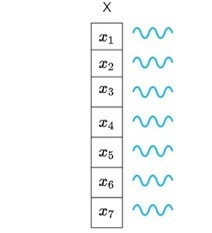
\includegraphics[width=0.85\textwidth]{Figures/jac_parallel}
 \caption{Parallel Jacobi Method}
 \label{fig:jac_par}
\end{subfigure}%
\begin{subfigure}{.5\textwidth}
 \centering
 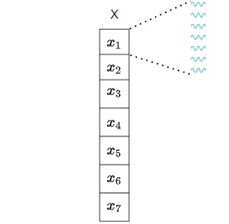
\includegraphics[width=1\textwidth]{Figures/row_based}
 \caption{Row Based Method}
 \label{fig:row_based}
\end{subfigure}
\caption{Parallel Threads}
\end{figure}


% ############################################################################
\subsection{Gauss-Seidel Method (Sequential version)}
% ############################################################################

The Gauss-Sidel method is an iterative method for solving linear equations \cite{7396262}. This  is also referred as the Liebmann method. The Gauss-Seidel and Jacobi methods are nearly identical. The only difference is that the Jacobian method is synchronous, whereas the GS method is asynchronous in nature. The Jacobi method calculaes any variable $x_i$ using the values obtained in the previous iteration, but the GS method always uses the most recently updated values during the iterative process. In other words, this method updates vector $X$ immediately after solving any equation $i$ (as given in formula\eqref{equ:gs}), but the Jacobian method updates vector $X$ only after each iteration. Thus, the GS method begins the approximation process far earlier than the Jacobi method. As a result, this method, even for enormous systems, can achieve convergence in very few iterations compared to the Jacobi method. Thus, this method overcame the Jacobi method's slow convergence issue. The variable vector $X$ is initialized with some initial values in this algorithm. Then, as demonstrated in the algorithm~\ref{alg:gauss_seidel_seq}, equation $i$ is solved as per formula~\eqref{equ:gs} and $X[i]$ is updated immediately. Here, variable $x_i$ is dependent on variables ${x_1, x_2,... x_{i-1}}$. These processes are carried out until convergence occurs.

\begin{subequations}\label{equ:gs}
\begin{align*}
x_i = \frac{b_i - \Sigma_{i \ne j}(a_{ij} \times x_j)}{a_{ii}}
\tag{\ref{equ:gs}}
\end{align*}
\end{subequations}

\begin{algorithm}
\DontPrintSemicolon 
\caption{Gauss Seidel (Sequential)}\label{alg:gauss_seidel_seq}
\SetKwInOut{Input}{input}
\SetKwInOut{Output}{output}
\Input{matrix A = coefficient matrix\\ vector B = constant vector  }
\Output{Solution vector X}
$X \gets (0,0,...,0)_n$\;
 \While{until convergence}{
  \For{$i \gets 0$ \KwTo $size$}{
   $X[i] \gets B[i]$\;
   \For{$j \gets 0$ \KwTo $size$}{
    \If{$i \ne j$}{
     $X[i] \gets X[[i] - (A[i][j] \times X[j])$\;
    }
   }
   $X[i] \gets X[i] / A[i][i]$ \Comment*[r]{Immediate update variable vector X}
  }
 }
\end{algorithm}


% ############################################################################
\subsection{Row-Based Method (Parallel version)}
% ############################################################################

As discussed above, the GS algorithm can achieve convergence in very few iterations, as it uses the most recently updated values. Thus, the calculation of variable $x_i$ is dependent on $x_1, x_2,...,x_{i-1}$. In other words, ${x_i}$ cannot be calculated without solving $x_{i-1}$. As a result, the GS algorithm cannot calculate all variables $x_1, x_2,...,x_{i-1}$ concurrently in a parallel system. The author proposed a row-based parallel method in the paper \cite{row-based}. In the formula ~\eqref{equ:gs}, the author calculated $\Sigma_{i \ne j}a_{ij}x_j^{(k-1)}$ this part in parallel system. There are $n-1$ multiplications and $n-1$ summations in expression~\eqref{equ:expression}. In a parallel system, $n$ threads are required to solve expression~\eqref{equ:expression}. Here $n$ denotes the number of equations. As seen in the figure ~\ref{fig:row_based}, $n$ threads are launched to solve the $i^{th}$ equation. Each thread $j$ multiplies $A[i][j]$ and $X[j]$ and saves the result in the multiplications vector. Then, as shown in the algorithm ~\ref{alg:row_based}, there will be a summation of multiplication vectors in the parallel system. And the value of $X[i]$ is updated based on the sum of the multiplication vector. These processes are carried out until convergence occurs.

\begin{subequations}\label{equ:expression}
\begin{align*}
\Sigma_{i \ne j}a_{ij}x_j^{(k-1)}
\tag{\ref{equ:expression}}
\end{align*}
\end{subequations}

\begin{algorithm}
\DontPrintSemicolon 
\SetKwBlock{DoParallel}{do in parallel}{end}
\caption{Row Based Parallel Method}\label{alg:row_based}
\SetKwInOut{Input}{input}
\SetKwInOut{Output}{output}
\Input{matrix A = coefficient matrix\\ vector B = constant vector  }
\Output{Solution vector X}
$X \gets (0,0,...,0)_n$\;
 \texttt{$multiplications \gets$ array of size X} \Comment*[r]{GPU Global Memory}
 \While{until convergence}{
  \For{$i \gets 0$ \KwTo $size$}{
   \DoParallel{
    $\texttt{(Copy matrix A and vector X in shared memory)}$
    $j \gets blockIdx.x \times blockDim.x + threadIdx.x$\;
    $multiplications[j] = A[i][j] \times X[j]$\;
   }
   \DoParallel{
    \texttt{Do sum of array multiplications}
   }
   \DoParallel{
    \texttt{(Only one CUDA thread)}\;
    $j \gets blockIdx.x \times blockDim.x + threadIdx.x$\;
    \If{$j \ne 0$}{
     $X[i] \gets (B[i] - multiplications[0])/A[i][i]$\;
    }
   }
  }
 }
\end{algorithm}


% ############################################################################
\subsection{Parallel Jacobi Gauss-Seidel Method}
% ############################################################################

So far, two iterative techniques have been discussed: the Jacobi and the Gauss-Seidel. While the Jacobi method can achieve a high degree of parallelization, it requires too many iterations to achieve convergence, and in the worst-case method, it becomes stuck and never achieves convergence for big systems. The GS method requires a small number of iterations to reach convergence, even for huge systems, but it is extremely difficult to apply in a parallel system because any variable $i$ is dependent on variable $i-1$. In other words , if good parallelization is desired, the time required for the algorithm to reach convergence must be compromised, and vice versa. In other words, the Jacobi and GS methods cannot accomplish both high parallelization and fast convergence.

\begin{algorithm}
\DontPrintSemicolon 
\SetKwBlock{DoParallel}{do in parallel}{end}
\caption{PJG Method}\label{alg:pjg}
\SetKwInOut{Input}{input}
\SetKwInOut{Output}{output}
\Input{matrix A = coefficient matrix\\ vector B = constant vector\\ P = block size  }
\Output{Solution vector X}
$X \gets (0,0,...,0)_n$\;
 \While{until convergence}{
    \For{$blockIndex \gets 0$ \KwTo $ceil(size/p)$}{
        \DoParallel{
            \texttt{(Copy matrix A, vector B and vector X in shared memory)}
            $threadId \gets blockIdx.x \times blockDim.x + threadIdx.x$\;
            
            \If{$threadId < P$}{
                $prediction \gets 0$\;
                $i \gets blockIndex \times P + threadId$\;
                \If{$i<size$}{
                    $prediction \gets B[i]$\;
                    \For{$j \gets 0$ \KwTo $size$}{
                        \If{$i \ne j$}{
                            $prediction \gets prediction - (A[i][j] \times X[j])$\;
                        }
                    }
                    $prediction \gets prediction / A[i][i]$\;
                }
            }
           $\texttt{(Synchronize threads)}$\;
           $X[i] \gets prediction$ \Comment*[r]{Update in global memory}
        }
        $blockIndex \gets blockIndex + 1$\;
    }
 }
\end{algorithm}

\noindent \\ To address this issue, the author of paper \cite{base-paper} developed a new method called the PJG (Parallel Jacobi Gauss-Seidel) method. The PJG method combines the Jacobi and GS methods. The author of the paper \cite{base-paper} combined the good characteristics of both methods to develop the PJG method. The good feature of the Jacobi method is that it updates variable vector X after every iteration, which is why the Jacobi method is very easy to implement in a parallel system. The advantage of the GS method is that after solving any variable $x i$, it immediately updates variable vector $X$ and uses the most recently updated values of variable vector $X$, which explains why convergence occurs very quickly. The PJG method divides equations into blocks of size p. All equations within the same block are solved simultaneously in a parallel system (a Jacobi method feature), and once one batch is solved, variable vector X is updated (a feature of the GS method). The remaining batches' equations will now use the updated vector X values. Due to the fact that all equations in the same batch size are independent of one another, they are solved parallely. After solving all equations in a batch, the variable vector X is updated. Thus, in comparison to the Jacobi method, there will now be more frequent updates to variable vector X. As a result, the PJG algorithm converges in a very few iterations. Therefore, the PJG algorithm achieves both high parallelism and convergence.

\begin{figure}[h]
\centering
\begin{subfigure}{.5\textwidth}
 \centering
 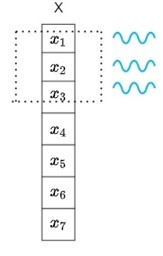
\includegraphics[width=0.6\textwidth]{Figures/pjg}
 \caption{Parallel Jacobi Gauss-Seidel Method}
 \label{fig:pjg}
\end{subfigure}%
\begin{subfigure}{.5\textwidth}
 \centering
 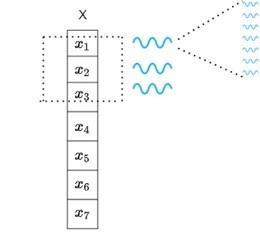
\includegraphics[width=1\textwidth]{Figures/pjg_dp}
 \caption{PJG with Dynamic Parallelization}
 \label{fig:pig_dp}
\end{subfigure}
\caption{Parallel Threads for PJG method}
\end{figure}

\noindent \\ To solve linear equations in a parallel system using the PJG method, $p$ threads are required. Initially variable vector X initialized with some values.     As shown in the figure ~\ref{fig:pjg}, each thread $i$ will solve equation $i$ in the batch. Once all equations have been solved in a batch, the variable vector X will be updated in the as shown in algorithm ~\ref{alg:pjg}. Then the next $p$ equations will be solved, and so on until all of the equations are solved. All of these processes will be repeated until the algorithm reaches convergence.
\\
\\
The primary objective of this research is to archive more parallelization in the PJG method. I hypothesised that by integrating the dynamic parallelization concept with the PJG method, the performance of the PJG method can be improved. To test this hypothesis, I have made appropriate changes in the PJG algorithm by applying the dynamic parallelization concept to it and then implementing it in a parallel environment. I have compared the performance of the PJG method with dynamic parallelization, with all the above algorithms discussed so far.


% ###########################################################################e
\section{Proposed Method} \label{proposed_method}
% ############################################################################

% ############################################################################
\subsection{Dynamic Parallelization} \label{dp}
% ############################################################################

In CUDA, a kernel is a function that runs on the GPU. Generally, the kernel is invoked by host code, but in some situations, more parallelization may be achieved by calling a kernel from another kernel. This is called "dynamic parallelization". A set of threads is called a "block" in CUDA. A grid is a set of blocks in the CUDA programming architecture. A kernel operates on a grid. A parent grid launches kernels known as child grids in CUDA Dynamic Parallelism. Certain properties and restrictions, such as the L1 cache/shared memory configuration and stack size, are inherited by a child grid from the parent grid. The most important thing to remember about dynamic parallelization is that any thread that meets a kernel launch will execute it. So, if the parent grid contains 128 blocks, each with 64 threads, there will be 8192 kernel launches. It can degrade the performance. It is critical to control the number of child kernels that are invoked. Grid launches are completely nested in dynamic parallelization. To put it another way, child grids are always completed before parent grids. There is no need for explicit synchronization. Exexution of dynamic parallelization is shown in figure~\ref{fig1}. If the parent kernel requires the results computed by the child kernel in order to conduct its own work, the parent kernel must explicitly synchronize in order to ensure that the child grid has finished execution before proceeding with the work.
\\
\\
A parent grid frequently relies on a child grid to read and write to global memory. To accomplish this, the CUDA Device Runtime ensures that the parent and child grids have a fully consistent view of global memory when the child starts and stops. In other words, if a parent writes in memory and then launches a child grid, CUDA will make sure that the child grid will see the value written by the parent grid and vice versa. This also means that if more than one child grid is run consecutively, any writes made by earlier child grids are seen by later child grids, even if no synchronization has occured between them. Memory consistancy is shown in figure`\ref{fig2}.

\begin{figure}[h]
\centering
 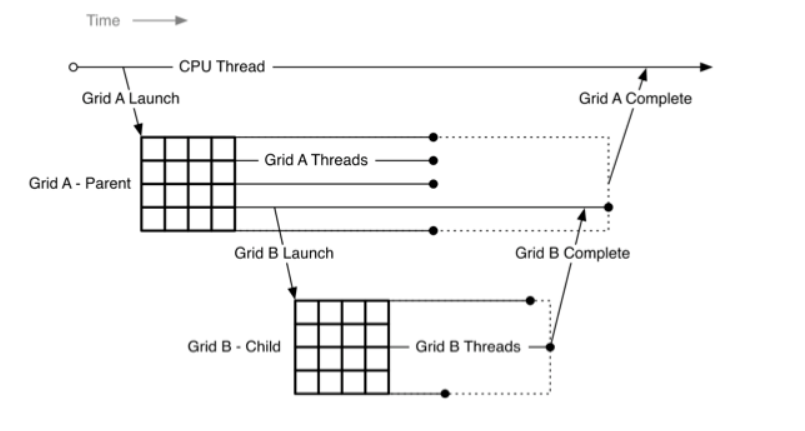
\includegraphics[width=0.6\textwidth]{Figures/figure1}
 \caption{Execution of dynamic parallelization}
 \label{fig1}
\end{figure}

\begin{figure}[h]
 \centering
 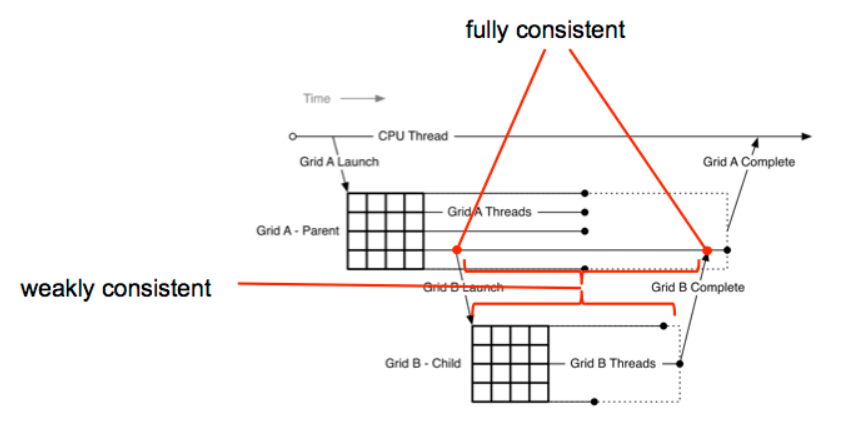
\includegraphics[width=1\textwidth]{Figures/figure2}
 \caption{Memory consistency}
 \label{fig2}
\end{figure}

During the experiment, it is observed that performance of the JPG algorithm degrades rather than improves. This is because kernel launching, whether parent or child, is a difficult process \href{https://developer.nvidia.com/blog/cuda-dynamic-parallelism-api-principles/}{[nvidia documentation]}. If child kernels do not extract much parallelism, then the child kernel launch overheads may cancel out any benefit. To overcome this, I implemented dynamic parallelism without the use of a nested kernel.


% ############################################################################
\subsection{The PJG algorithm with dynamic parallelization} \label{dp}
% ############################################################################

As we have discussed above, dynamic parallelization is a nested kernel execution.  As shown in the figure ~\ref{fig:pig_dp}, thread $i$ solves the $i^{th}$ equation in block. In other words, thread $i$ calculates the expression ~\ref{equ:expression} in formula \ref{equ:gs} for linear equation $i$ . All threads perform these calculations simultaneously in order to solve all of the equations contained within the same block. For block of size p, the PJG algorithm requires p threads. The initial idea was to invoke $n$ child threads from every $p$ parent thread, as shown in the figure ~\ref{fig:pig_dp}. All these child threads of parent thread $i$, calculate expression ~\ref{equ:expression} in formula \ref{equ:gs} for equation $i$, in a parallel environment. However, as noted previously, executing a child kernel is a difficult and time consuming process. As a result, I attempted to simulate dynamic parallelization without using a nested kernel to avoid this limitation.

\begin{algorithm}
\DontPrintSemicolon 
\SetKwBlock{DoParallel}{do in parallel}{end}
\caption{PJG Method (Dynamic Parallelization)}\label{alg:pjg_dp}
\SetKwInOut{Input}{input}
\SetKwInOut{Output}{output}
\Input{matrix A = coefficient matrix\\ vector B = constant vector\\ P = block size  }
\Output{Solution vector X}
$X \gets (0,0,...,0)_n$\;
\texttt{$multiplications \gets$ matrix of dimensions P X size} \Comment*[r]{GPU Global Memory}
 \While{until convergence}{
    \For{$blockIndex \gets 0$ \KwTo $ceil(size/p)$}{
        \DoParallel{
            \texttt{(Copy matrix A, vector B and vector X in shared memory)}
            $threadId \gets blockIdx.x \times blockDim.x + threadIdx.x$\;
            $equationId \gets floor(threadId/size)$\;
            
            \If{$equationId < P$}{
                $i \gets blockIndex \times P + equationId$\;
                $j \gets threadId \Mod {size}$\;
                
                \uIf{$i == j$}{
                    $multiplications[equationId][j] \gets 0$\;
                }
                \Else{
                    $multiplications[equationId][j] \gets A[i][j] \times X[j]$\;
                }
            }
        }
        \DoParallel{
            $\texttt{(Parallel summation of elements of each row in multiplications matrix)}$
        }
        \DoParallel{
             \texttt{(P threads)}\;
             \texttt{(Copy matrix A, vector B and matrix multiplications in shared memory)}
            
            $threadId \gets blockIdx.x \times blockDim.x + threadIdx.x$\;
            $equationId \gets floor(threadId/size)$\;
            
            \If{$threadId < P$}{
                $i \gets blockIndex \times P + threadId$\;
                $X[i] \gets \frac{B[i] - sum(multiplications[threadId])}{A[i][i]}$\;
            }
        }
        $blockIndex \gets blockIndex + 1$\;
    }
 }
\end{algorithm}

\noindent \\Instead of executing $p$ parent threads first and then $n$ child threads from every $p$ parent thread, one can execute $p \times  n$ threads from host code only. Then every thread is assigned the equation id as shown in the algorithm ~\ref{alg:pjg_dp}. The equation id $i$ indicates that the thread is solving $i^{th}$ equation in the block. So, for the first $n$ threads, the equation id will be $0$, then for the next $n$ threads, it will be $1$ and so on. For each thread, $i$ and $j$ variables are assigned as shown in the algorithm ~\ref{alg:pjg_dp}. An variable $i$ indicates that thread is solving equation $i$ and variable $j$ indicates that thread multiple $A[i][j]$ and $X[i]$. All these multiplications are stored in a matrix named "multiplications". After that, every thread will do a summation of each row of multiplications matrix simultaneously, and then variable vector $X$ will be updated. These operations are performed until the algorithm achieves convergence. Such that dynamic parallization is simulated without using nested kernel execution.

% ############################################################################
\section{Experiment} \label{expermient}
% ############################################################################

% ############################################################################
\subsection{Hardware and Software Configuration} \label{result}
% ############################################################################

The computer hardware used in this experiment is equipped with used an NVIDEA T4 GPU. The GPU features 320 tensor cores and 2560 CUDA cores. This GPU has 16 GB of GDDR6 global memory. Cuda is used to implement algorithms in GPU. Cuda is an extension in C++.

% ############################################################################
\subsection{Simulation Settings} \label{simulation_settings}
% ############################################################################

To provide a comprehensive performance report, simulation settings cover two types of systems with liner equations: large systems and small systems. A total of seven algorithms were used in this experiment. Those algorithms are the Jacobi Algorithm, the Jacobi algorithm with a parallel version of the Jacobi algorithm, the GS algorithm, the Row Based method, the sequantial version of the PJG method, the parallel version of the PJG method, and the proposed method (the PJG method with dynamic parallelization). All algorithms are tested on the same inputs.
\\
\\
The first test is conducted with a small system of linear equations. A total of 50 equations are used. The block size is 10 for the PJG method. The second test is conducted with a large system of linear equations. A total of 1000 equations are used. The block size is 35 for the PJG method. The third test is also conducted with 1000 linear equations and with block size 35. But in this particular test, all algorithms are forced to run for 1000 iterations instead of until convergence is achieved.

% ############################################################################
\subsection{Results} \label{results}
% ############################################################################

\begin{table}[h]
\centering
\begin{tabular}{|l|l|l|l|}
\hline
Method                                                                   & \begin{tabular}[c]{@{}l@{}}Time\\ (Seconds)\end{tabular} & Iterations \\ \hline
Jacobi            & 0.0125762   & 478 \\ \hline
Jacobi (Parallel) & 0.0268081   & 478 \\ \hline
Gauss Seidel      & 0.0001888   & 7   \\ \hline
\begin{tabular}[c]{@{}l@{}}Row Based \\ Parallel Method\end{tabular}     & 0.00842755                                               & 7          \\ \hline
PJG (Sequential)  & 0.000267712 & 9   \\ \hline
PJG (Parallel)    & 0.00077216  & 9   \\ \hline
\begin{tabular}[c]{@{}l@{}}PJG \\ (Dynamic Parallelization)\end{tabular} & 0.00100070906                                            & 9          \\ \hline
\end{tabular}
\caption{\\ Iteraions : until convergence \\ Number of equations : 50 \\ Block size : 10}
\label{table:1}
\end{table}

\begin{table}[h]
\centering
\begin{tabular}{|l|l|l|l|}
\hline
Method                                                                   & \begin{tabular}[c]{@{}l@{}}Time\\ (Seconds)\end{tabular} & Iterations \\ \hline
Jacobi            & 99.802    & 1000 (no convergence) \\ \hline
Jacobi (Parallel) & 5.69737   & 1000 (no convergence) \\ \hline
Gauss Seidel      & 0.0992823 & 10                    \\ \hline
\begin{tabular}[c]{@{}l@{}}Row Based \\ Parallel Method\end{tabular}     & 0.0930212                                                & 10         \\ \hline
PJG (Sequential)  & 0.267712  & 10                    \\ \hline
PJG (Parallel)    & 0.056479  & 10                    \\ \hline
\begin{tabular}[c]{@{}l@{}}PJG \\ (Dynamic Parallelization)\end{tabular} & 0.039485                                                 & 10         \\ \hline
\end{tabular}
\caption{\\ Iteraions : until convergence \\ Number of equations : 1000 \\ Block size : 35}
\label{table:2}
\end{table}


\begin{table}[h]
\centering
\begin{tabular}{|l|l|l|l|}
\hline
Method                                                                   & \begin{tabular}[c]{@{}l@{}}Time\\ (Seconds)\end{tabular} \\ \hline
Jacobi                                                                   & 5.562                                                    \\ \hline
Jacobi (Parallel)                                                        & 0.270                                                    \\ \hline
Gauss Seidel                                                             & 5.518                                                    \\ \hline
\begin{tabular}[c]{@{}l@{}}Row Based \\ Parallel Method\end{tabular}     & 3.389                                                    \\ \hline
PJG (Sequential)                                                         & 5.549                                                    \\ \hline
PJG (Parallel)                                                           & 0.770                                                   \\ \hline
\begin{tabular}[c]{@{}l@{}}PJG \\ (Dynamic Parallelization)\end{tabular} & 0.587                                                    \\ \hline
\end{tabular}
\caption{\\ Iteraions : 1000 \\ Number of equations : 1000 \\ Block size : 35}
\label{table:3}
\end{table}


Table ~\ref{table:1} summarizes the results of the first test (small system of linear equations). The Jacobi method required 478 iterations to solve 50 linear equations, whereas the GS and PJG methods required just 7 and 9 iterations, respectively. A critical point to note here is that all parallel algorithms take longer than their sequential counterparts for small system. This is because the degree of parallelization highly depends on the number of equations. If the number of equations is small, kernel launch and data operations cancel out any benefit gained by parallel operations.
\\
\\
Results for the second test (a large system of linear equations) are shown in Table ~\ref{table:2}. The number of equations is 1000, and the block size for the PJG is 35. The Jacobi method (parallel version) achieved a 17.5x speedup compared to its sequential version. But even after 1000 iterations, it does not solve equations. All other methods take only 10 iterations to solve 1000 linear equations. The GS algorithm took almost the same time in the parallel and sequential versions. No significant speedup was observed in this test for the GS algorithm. The proposed algorithm (the PJG with dynamic parallelization) takes the least amount of time of all the other algorithms. The PJG algorithm (parallel version) and the proposed algorithm achieved 5.74x and 6.78x speedup compared to the PJG (sequential version). When compared to the GS method, the proposed method achieved a 2.5x speedup, while the PJG method (parallel version) achieved a 1.75x speedup. Here, there is no significant performance enhancement observed, this is because the GS algorithm and the PJG algorithm solved 1000 equations in just 10 iterations.
\\
\\
Results for the test (large system but all algorithms are forced to run for 1000 iterations) are shown in table ~\ref{table:3}. The number of equations is 1000 and the block size is 35 for the PJG method. The Jacobi algorithm achieved a 20.6x speedup, but in this test also, the algorithm does not solve the equations after 1000 iterations. The proposed algorithm took the least time (the Jacobi method does not solve equations, so its results are not considered). The PJG method (parallel version) and the proposed method achieved 7.2x and 9.45x speedup, respectively, when compared with the sequential version of the PJG method. When compared to the sequential version of the GS method, the parallel version of the PJG method achieved a 7.1x speedup, while the proposed method achieved a 9.4x speedup.

% ############################################################################
\subsection{Conclusion} \label{conclusion}
% ############################################################################

In this research work, I have tried to improve the performance of the PJG method by applying dynamic parallelization. The proposed method achieved a 9.45x speedup compared to the sequential PJG method, which is higher than the 7.2x speedup achieved by the parallel PJG method. The proposed method achieved a 9.4x speedup compared to the GS method. Additionally, I have compared the performance of various algorithms like the Jacobi algorithm, the GS algorithm, and the PJG algorithm by executing them on the GPU. The Jacobi method achieved the highest speedup, which is 20.6x, but it didn't achieve convergence. The GS method achieved good convergence, but it did not achieve significant speedup. The PJG method achieved good parallelization and convergence as well. Further work will focus on developing an algorithm for the proposed method to implement it in a distributed memory architecture.

% ############################################################################
% Bibliography
% ############################################################################
\bibliographystyle{plain}
\bibliography{final_paper_ref
}     %loads my-bibliography.bib

% ============================================================================
\end{document}
% ============================================================================
